\documentclass[10pt, aspectratio = 169, handout]{beamer} % handout

\usepackage{amsmath}
\usepackage{fontawesome} 
\usepackage{ragged2e}
\usepackage{color}
\usepackage{tikz}
\usepackage{soul}
\usepackage{xcolor}
\usepackage{import}
\usepackage{xifthen}
\usepackage{pdfpages}
\usepackage{transparent}
\usepackage{soul}
\usepackage[mathscr]{euscript}
\usepackage{dsfont}
\usepackage{caption}

\usetikzlibrary{shapes, backgrounds, plotmarks}

% Curly D [euscript]
\DeclareSymbolFont{rsfs}{U}{rsfs}{m}{n}
\DeclareSymbolFontAlphabet{\mathscrsfs}{rsfs}

\usetheme[]{metropolis}
\usecolortheme[]{wolverine}

\usefonttheme{serif}
\setbeamercovered{transparent = 0.5}

\setbeamertemplate{theorems}[numbered]

\definecolor{title-bg}{RGB}{240, 240, 240}
\definecolor{title-fg}{RGB}{128, 113, 93}
\definecolor{my-red}{RGB}{254, 132, 135}
\definecolor{my-blue}{RGB}{59, 180, 252}
\definecolor{my-green}{RGB}{125, 221, 149}
\definecolor{titles}{RGB}{0, 0, 122}
\setbeamercolor{block title}{fg = title-fg, bg = title-bg}
\setbeamercolor{header-color}{fg = title-fg, bg = title-bg}
\setbeamercolor{background canvas}{bg = white}

\let\oldtextbf\textbf
\renewcommand\textbf[1]{\textcolor{titles}{\oldtextbf{#1}}}

\DeclareCaptionLabelSeparator{pers}{\textcolor{titles}{: }}
\captionsetup{labelsep=pers}
\renewcommand{\thetable}{\textcolor{titles}{\arabic{table}}}
\captionsetup[table]{name=\textcolor{titles}{Table}}
\renewcommand{\thefigure}{\textcolor{titles}{\arabic{figure}}}
\captionsetup[figure]{name=\textcolor{titles}{Figure}}

\newcommand{\backupbegin}{
   \newcounter{finalframe}
   \setcounter{finalframe}{\value{framenumber}}
}
\newcommand{\backupend}{
   \setcounter{framenumber}{\value{finalframe}}
}

\setbeamertemplate{footline}{%
	\leavevmode%
	\hbox{%
		\begin{beamercolorbox}[wd = 0.800\textwidth, ht = 4ex, dp = 2ex, left]{}%
			\hspace{4pt} \texttt{Extended Excess Hazard Models for Spatially Dependent Survival Data}
		\end{beamercolorbox}%
		\begin{beamercolorbox}[wd = 0.120\textwidth, ht = 4ex, dp = 2ex, center]{}%
			\raisebox{-1pt}{\insertslidenavigationsymbol~\insertsectionnavigationsymbol}
		\end{beamercolorbox}%
		\begin{beamercolorbox}[wd = 0.080\textwidth, ht = 4ex, dp = 2ex, center]{}%
			\texttt{\insertframenumber~/~\inserttotalframenumber}
		\end{beamercolorbox}%
	}%
}%


\author{André Victor Ribeiro Amaral}

\begin{document}
	\AtBeginSection{}
	\metroset{block = fill}
	{
		\usebackgroundtemplate{
    		\hspace{6pt}
    		
\includegraphics[width=0.35\textwidth]{Images/KAUST_logo.png}
		}

        \begin{frame}[t]
            
            \centering
            \vspace{55pt}
            \textbf{{\large \usebeamercolor[fg]{frametitle}Extended Excess Hazard Models for Spatially Dependent Survival Data}} \\
            \vspace{15pt}
            {\normalsize André V.\hspace{1pt} Ribeiro Amaral${}^{\hspace{-1pt}~\dagger}$}\\
            {\scriptsize\texttt{\href{mailto:andre.ribeiroamaral@kaust.edu.sa}{andre.ribeiroamaral@kaust.edu.sa}}} \\
            \vspace{15pt}
            {\small King \hspace{-1pt}Abdullah\hspace{-1pt} University \hspace{-1pt}of Science\hspace{-1pt} and \hspace{-1pt}Technology \hspace{-2pt}(KAUST)}\\
            {\small Geospatial Statistics and Health Surveillance Research Group} \\ \vspace{15pt}

            \begin{flushleft} 
            {\small ${}^{\dagger\hspace{1pt}}$Joint work with Francisco Javier Rubio, Manuela Quaresma, Francisco J. Rodr\'iguez-Cort\'es, and Paula Moraga.}
            \end{flushleft}
        \end{frame}
  	}

	\begin{frame}[t]
		\frametitle{Introduction}
		\justifying

        {\textbf{\textcolor{red}{Goal:}}} Under the ``\ul{relative survival framework},'' we aim at \ul{proposing a general parametric class of frailty models} and inference tools that account for spatial dependence (and \ul{investigate geographical inequalities in England})\footnote{\justifying Amaral, A. V. R., Rubio, F. J., Quaresma, M.,  Rodr\'iguez-Cort\'es, F. J., and Moraga, P. (2023). Extended Excess Hazard Models for Spatially Dependent Survival Data. arXiv. \url{https://arxiv.org/abs/2302.09392}.}.

        \pause

        When modeling survival data, we may work under three different frameworks
		\begin{enumerate}
			\justifying
			\item \textbf{Overall survival framework:} no distinction is made among the possible causes of death. This is not useful when comparing populations.
			\item \textbf{Cause-specific framework:} used when the cause of death is known. For certain diseases and locations, this information may not be available.
			\item \textbf{\ul{Relative survival framework}:} used when we can decompose the hazard function into ``hazard associated with other causes'' and ``hazard associated with some specific disease.''  Useful when comparing populations.
		\end{enumerate}

	\end{frame}

    \begin{frame}[t]
		\frametitle{Introduction}
		\justifying
		Let $T_1, \cdots, T_n$ represent the time-to-death for $n$ individuals, such that $T_i \overset{\text{i.i.d.}}{\sim} G$, $\forall i$.
		
		In that case, we are interested in the following functions
		\begin{itemize}
			\justifying
			\item Survival function: $S(t) = \mathbb{P}(T > t) = 1 - F(t)$, such that $F(t)$ is the CDF.
			\item Hazard function:
			\begin{align*}
				h(t) = \lim_{dt \to 0} \frac{\mathbb{P}(t \leq T < t + dt | T \geq t)}{dt} = \frac{f(t)}{S(t)} = -\frac{d \log S(t)}{dt},
			\end{align*}
		    such that $f(t)$ is the PDF. $h(t)$ can be interpreted as the rate of death at $t$. The hazard functions is also used to characterize the distribution of $T$.
		    \item Cumulative Hazard function: $H(t) = \int_0^t h(s)ds$, such that $S(t) = \exp\left\{-H(t)\right\}$.
		\end{itemize}
	\end{frame}
	
	\begin{frame}[t]
		\frametitle{Relative survival framework}
		\justifying
    	Under the \ul{relative survival framework}, and assuming we are analyzing cancer-diagnosed patients,
    	\begin{align*}
        	h(t; \mathbf{x}) = h_{\text{O}}(\text{age} + t) + h_{\text{E}}(t; \mathbf{x}),~ t \geq 0,
    	\end{align*}
    	where $h_{\text{O}}$ is the hazard associated with other causes of death, and $h_{\text{E}}$ is associated with cancer. $h_{\text{E}}$ is also known as excess hazard. Also, ``age'' is the patient's age when diagnosed, and $\mathbf{x}$ is a vector of risk factors.
    	
    	As $h_{\text{O}}$ is usually not known in practice, we approximate it by the population hazard $h_{\text{P}}$ (estimated by life-tables). In that way,
    		\begin{align*}
    			h(t; \mathbf{x}, \mathbf{z}) = h_{\text{P}}(\text{age} + t; \mathbf{z}) + h_{\text{E}}(t; \mathbf{x}),~ t \geq 0,
    		\end{align*}
    	such that $\mathbf{z} \subseteq \mathbf{x}$ is a vector of patient characteristics (e.g., age, sex, race, etc.).
	\end{frame}
	
	\begin{frame}[t]
		\frametitle{Relative survival framework}
		\justifying
        When comparing populations using models fitted under the relative survival framework, people usually refer to the \ul{net survival}, that is
		\begin{align*}
			S_{\text{N}}(t; \mathbf{x}) = \exp\left\{-\int^t_0 h_{\text{E}}(s; \mathbf{x})ds\right\},
		\end{align*}
		where $h_{\text{E}}$ is the excess hazard. Alternatively, we can report the population net survival
		\begin{align*}
			S_{\text{N}}(t) = \frac{1}{m}\sum_{i = 1}^{m}S_{\text{N}}(t; \mathbf{x}_i),
		\end{align*}
        where $\{\mathbf{x}_i\}_{i=1}^m$ represents the set of covariates associated to the (sub-)population of interest.
	\end{frame}

    \begin{frame}[t]
		\frametitle{Excess hazard model}
		\justifying
        Let $t_{ij}$ be the observed survival times in the $i$-th region for the $j$-th patient, and $\delta_{ij}$ be the censoring indicators. Then, the model for $h_\text{E}(\cdot)$ is
        
        \vspace{-12pt}

        \begin{align} \label{eq:exc-haz}
            h_{\text{E}}(t; \mathbf{x}_{ij} \mid \boldsymbol{\theta}, \boldsymbol{\alpha}, \boldsymbol{\beta}, \boldsymbol{\gamma}, \tilde{u}_i, u_i) = h_0(t \exp\{\tilde{\mathbf{x}}_{ij}^{\top} \boldsymbol{\alpha} + \tilde{u}_i\} \mid  \boldsymbol{\theta}) \exp\{\mathbf{s}_{ij}^{\top} \boldsymbol{\gamma} + \mathbf{x}_{ij}^{\top} \boldsymbol{\beta} + u_i\},
        \end{align}

        where $h_0(\cdot \mid \boldsymbol{\theta})$ is the baseline function (defined through a parametric distribution), $\boldsymbol{\theta}$ represents the corresponding parameters, $\tilde{\mathbf{x}}_{ij} \subseteq \mathbf{x}_{ij}$, such that $\tilde{\mathbf{x}}_{ij} \in \mathbb{R}^{\tilde{p}}$ and $\mathbf{x}_{ij} \in \mathbb{R}^p$, $\boldsymbol{\alpha} = (\alpha_1, \cdots, \alpha_{\tilde{p}})^{\top}$, and $\boldsymbol{\beta} = (\beta_1, \cdots, \beta_{p})^{\top}$. Also, $\mathbf{s}_{ij} = ({s_{ij1}}^{\top}, \cdots, {s_{ijq}}^{\top})^{\top} \in \mathbb{R}^q$ and $\boldsymbol{\gamma} = (\gamma_1, \cdots, \gamma_q)^{\top}$, where $q = \sum_{\ell = 1}^{k}q_{\ell}$, such that $q_{\ell}$ is the dimension of $s_{ij\ell}$, and $s_{ij\ell}$ is the spline expansion of a (continuous) covariate $x_{ij\ell}$. 

        \vspace{5pt}
        
        The random effects will follow $\tilde{\mathbf{u}} = (\tilde{u}_i, \cdots, \tilde{u}_r)^{\top} \sim \tilde{G}$ and $\mathbf{u} = \hspace{-1pt}(u_1, \cdots, u_r)^{\top} \sim G$, such that $\tilde{G}$ and $G$ are spatially (in)dependent models (e.g., IID, ICAR, BYM2, etc.).

	\end{frame}

     \begin{frame}[t]
        \frametitle{Relative Survival Relative Survival Spatial General Hazard (RS-SGH)}
        \justifying
        
        Notice that \textcolor{titles}{Model \eqref{eq:exc-haz}}---name it ``Relative Survival Spatial General Hazard'' (RS-SGH) model---generalizes the following approaches

        \begin{table}[]
            %\resizebox{\textwidth}{!}{%
                \caption{\justifying All possible model extensions based on the Relative Survival Spatial General Hazard (RS-SGH) approach.}
                \label{tab:models-surv}
                \begin{tabular}{l | c | l | c }
                Name & Description & Name & Description  \\ \hline 
                RS-SGH-I &  $\tilde{\mathbf{u}} = \mathbf{0}$& RS-GH & $\tilde{\mathbf{u}} = \mathbf{u} = \mathbf{0}$ \\
                RS-SGH-II &  $\tilde{\mathbf{u}} = \mathbf{u}$& RS-PH & $\tilde{\mathbf{u}} = \mathbf{u} = \mathbf{0}, \boldsymbol{\alpha} = \mathbf{0}$ \\
                RS-MEPH &  $\tilde{\mathbf{u}} = \mathbf{0}, \boldsymbol{\alpha} = \mathbf{0}$& RS-AFT & $\tilde{\mathbf{u}} = \mathbf{u} = \mathbf{0}, \boldsymbol{\alpha} = \boldsymbol{\beta}$ \\
                RS-MEAFT &  $\tilde{\mathbf{u}} = \mathbf{u}, \boldsymbol{\alpha} = \boldsymbol{\beta}$& RS-AH&  $\tilde{\mathbf{u}} = \mathbf{u} = \mathbf{0}, \boldsymbol{\beta} = \mathbf{0}$ \\
                \end{tabular}%
            %}
        \end{table}

    \end{frame}

    \begin{frame}[t]
    	\frametitle{Inference}
    	\justifying

        Let $\mathcal{D} = \{(t_{ij}, \delta_{ij}, \mathbf{x}_{ij}, \mathbf{z}_{ij}); \, i = 1, \ldots, r, \text{ and } j = 1, \ldots, n_i\}$ be the observed data. In that case, the likelihood function for the vector of unknown parameters can be written as proportional to
        \begin{align} \label{eq:like}
            \prod_{i = 1}^{r}\prod_{j = 1}^{n_i} \left\{h_{\text{P}}(\text{age}_{ij} + t_{ij}; \mathbf{z}_{ij}) + h_{\text{E}}(t_{ij}; \mathbf{x}_{ij} \mid  \boldsymbol{\xi}, \tilde{u}_i, u_i)\right\}^{\delta_{ij}} \exp\{-H_{\text{E}}(t_{ij}; \textbf{x}_{ij} \mid  \boldsymbol{\xi}, \tilde{u}_i, u_i)\},
        \end{align}
        where $h_{\text{P}}(\text{age}_{ij} + t_{ij}; \mathbf{z}_{ij})$ is obtained from the life tables. 

        \vspace{5pt}
        
        From \textcolor{titles}{Equation \eqref{eq:like}}, notice that the only term in the likelihood function that distinguishes an overall survival model from a relative survival model is $h_{\text{P}}(\text{age}_{ij} + t_{ij}; \mathbf{z}_{ij})$; thus, by setting it to zero, we could also retrieve the overall survival framework.
            
    \end{frame}

    \begin{frame}[t]
		\frametitle{Implementation}
		\justifying
		As \textcolor{titles}{Model \eqref{eq:exc-haz}} is fully parametric, we will set the baseline $h_0(\cdot)$ structure as\vspace{-6pt}
		\begin{enumerate}
			\item Log-normal,
			\item Log-logistic,
			\item Power \hspace{-1pt}Generalized \hspace{-1pt}Weibull \hspace{-1pt}(not \hspace{-1pt}Weibull, due to \hspace{-1pt}non-identifiability \hspace{-1pt}issues),
			\item Gamma (it is tricky to fit, since it depends on a special function), and
			\item Generalized Gamma (same issues as for the Gamma).
		\end{enumerate}

        \pause
			
		And the random effects $\tilde{\mathbf{u}} = (\tilde{u}_i, \cdots, \tilde{u}_r)^{\top}\hspace{-3pt}$ and $\mathbf{u} = \hspace{-1pt}(u_1, \cdots, u_r)^{\top}\hspace{-3pt}$ will be set as
		\begin{enumerate}
			\item IID model; i.e., $\tilde{u}_i \overset{\text{i.i.d.}}{\sim}\text{Normal}(0, \sigma_{\tilde{u}}^2)$, $\forall i$ (same for $\tilde{\mathbf{u}}$),
			\item Intrinsic Conditional Autoregressive (ICAR) model, or
			\item Besag-York-Mollié (BYM2) model.
		\end{enumerate}
		
	\end{frame}
	
	\begin{frame}[t]
		\frametitle{Implementation}
		\justifying
        \begin{table}[!ht]
        	\caption{\justifying Implemented models based on the baseline distributions and the random effects structures.}
        	\resizebox{\textwidth}{!}{%
        	    \centering
        		\begin{tabular}{ c | c | l | l |  c |c | l | l | c | c | l | l | c | c | l | l | c | c | l | l }
        		\#  & Dist.& Model      & R.E. & \#  & Dist. & Model      & R.E. & \#  & Dist. & Model      & R.E. & \#  & Dist. & Model      & R.E. & \#  & Dist. & Model      & R.E. \\ \hline
        		01 & LN   & RS-SGH    & BYM2 & 20 & LL    & RS-SGH    & BYM2 & 39 & PGW   & RS-SGH    & BYM2 & 58 & GAM   & RS-SGH    & BYM2 & 77 & GG    & RS-SGH    & BYM2 \\
        		02 & LN   & RS-SGH    & ICAR & 21 & LL    & RS-SGH    & ICAR & 40 & PGW   & RS-SGH    & ICAR & 59 & GAM   & RS-SGH    & ICAR & 78 & GG    & RS-SGH    & ICAR \\  
        		03 & LN   & RS-SGH    & IID  & 22 & LL    & RS-SGH    & IID  & 41 & PGW   & RS-SGH    & IID  & 60 & GAM   & RS-SGH    & IID  & 79 & GG    & RS-SGH    & IID  \\  
        		04 & LN   & RS-SGH-I  & BYM2 & 23 & LL    & RS-SGH-I  & BYM2 & 42 & PGW   & RS-SGH-I  & BYM2 & 61 & GAM   & RS-SGH-I  & BYM2 & 80 & GG    & RS-SGH-I  & BYM2 \\
        		05 & LN   & RS-SGH-I  & ICAR & 24 & LL    & RS-SGH-I  & ICAR & 43 & PGW   & RS-SGH-I  & ICAR & 62 & GAM   &  RS-SGH-I & ICAR & 81 & GG    & RS-SGH-I  & ICAR \\
        		06 & LN   & RS-SGH-I  & IID  & 25 & LL    & RS-SGH-I  & IID  & 44 & PGW   & RS-SGH-I  & IID  & 63 & GAM   & RS-SGH-I  & IID  & 82 & GG    & RS-SGH-I  & IID  \\
        		07 & LN   & RS-SGH-II & BYM2 & 26 & LL    & RS-SGH-II & BYM2 & 45 & PGW   & RS-SGH-II & BYM2 & 64 & GAM   & RS-SGH-II & BYM2 & 83 & GG    & RS-SGH-II & BYM2 \\
        		08 & LN   & RS-SGH-II & ICAR & 27 & LL    & RS-SGH-II & ICAR & 46 & PGW   & RS-SGH-II & ICAR & 65 & GAM   & RS-SGH-II & ICAR & 84 & GG    & RS-SGH-II & ICAR \\
        		09 & LN   & RS-SGH-II & IID  & 28 & LL    & RS-SGH-II & IID  & 47 & PGW   & RS-SGH-II & IID  & 66 & GAM   & RS-SGH-II & IID  & 85 & GG    & RS-SGH-II & IID  \\
        		10 & LN   & RS-MEPH    & BYM2 & 29 & LL    & RS-MEPH    & BYM2 & 48 & PGW   & RS-MEPH    & BYM2 & 67 & GAM   & RS-MEPH    & BYM2 & 86 & GG    & RS-MEPH    & BYM2 \\  
        		11 & LN   & RS-MEPH    & ICAR & 30 & LL    & RS-MEPH    & ICAR & 49 & PGW   & RS-MEPH    & ICAR & 68 & GAM   & RS-MEPH    & ICAR & 87 & GG    & RS-MEPH    & ICAR \\
        		12 & LN   & RS-MEPG    & IID  & 31 & LL    & RS-MEPH    & IID  & 50 & PGW   & RS-MEPH    & IID  & 69 & GAM   & RS-MEPG    & IID  & 88 & GG    & RS-MEPG    & IID  \\
        		13 & LN   & RS-MEAFT   & BYM2 & 32 & LL    & RS-MEAFT   & BYM2 & 51 & PGW   & RS-MEAFT   & BYM2 & 70 & GAM   & RS-MEAFT   & BYM2 & 89 & GG    & RS-MEAFT   & BYM2 \\
        		14 & LN   & RS-MEAFT   & ICAR & 33 & LL    & RS-MEAFT   & ICAR & 52 & PGW   & RS-MEAFT   & ICAR & 71 & GAM   & RS-MEAFT   & ICAR & 90 & GG    & RS-MEAFT   & ICAR \\
        		15 & LN   & RS-MEAFT   & IID  & 34 & LL    & RS-MEAFT   & IID  & 53 & PGW   & RS-MEAFT   & IID  & 72 & GAM   & RS-MEAFT   & IID  & 91 & GG    & RS-MEAFT   & IID  \\
        		16 & LN   & RS-GH      & ---  & 35 & LL    & RS-GH      & ---  & 54 & PGW   & RS-GH      & ---  & 73 & GAM   & RS-GH      & ---  & 92 & GG    & RS-GH      & ---  \\
        		17 & LN   & RS-PH      & ---  & 36 & LL    & RS-PH      & ---  & 55 & PGW   & RS-PH      & ---  & 74 & GAM   & RS-PH      & ---  & 93 & GG    & RS-PH      & ---  \\ 
        		18 & LN   & RS-AFT     & ---  & 37 & LL    & RS-AFT     & ---  & 56 & PGW   & RS-AFT     & ---  & 75 & GAM   & RS-AFT     & ---  & 94 & GG    & RS-AFT     & ---  \\
        		19 & LN   & RS-AH      & ---  & 38 & LL    & RS-AH      & ---  & 57 & PGW   & RS-AH      & ---  & 76 & GAM   & RS-AH      & ---  & 95 & GG    & RS-AH      & ---  
        		\end{tabular}%
        	}
        	\label{tab:all-models}
        \end{table}

        \vspace{-7pt}

        Code \hspace{-1pt}implementation \hspace{-1pt}is available on \url{https://github.com/avramaral/relative\_survival}.
        
	\end{frame}

    \begin{frame}[t]
		\frametitle{Model selection}
		\justifying

        To compare the fitted models, we will use a leave-one-out cross validation (LOO CV) procedure. That is, we will use the likelihood evaluated at the parameters' posterior samples as a goodness-of-fit measure.

        \vspace{5pt}
        
        Under the Bayesian framework, the LOO estimate of out-of-sample predictive fit will be computed as
        \begin{align*}
            \text{elpd}_{\text{LOO}} &= \sum_{i = 1}^{r}\sum_{j = 1}^{n_i} \log\left[\pi(t_{ij}\mid\mathbf{t}_{-{ij}})\right],
        \end{align*}
        where $\pi(t_{ij} \mid \mathbf{t}_{-{ij}})$ is the LOO predictive density given $\mathbf{t}_{-ij}$, such that $\mathbf{t}_{-ij}$ corresponds to the vector of all observed time points, except $t_{ij}$. 

        \vspace{5pt}
        
        As a remark, the larger $\widehat{\text{elpd}}_{\text{PSIS-LOO}}$ (the estimate for $\text{elpd}_{\text{LOO}}$), the better.

	\end{frame}

    \begin{frame}[t]
		\frametitle{Applications}
		\justifying

        We will analyze a data set that contains survival information about male and female patients diagnosed with colon cancer between 2015 and 2016 in England.
        
        We will present two case studies \pause
        \begin{enumerate} \justifying
            \item Patients in all England with spatial structure defined in two different manners
            \vspace{5pt} \
            \begin{enumerate}
                \item Based on the administrative boundaries given by the Government Office Regions.
                \item Based on the health boundaries determined by the Cancer Alliances.
            \end{enumerate} \pause
            \vspace{5pt}
            \item Patients diagnosed with colon cancer in London. However, their locations (according to the London Clinical Commissioning Groups), will be defined based on
            \vspace{5pt}
            \begin{enumerate}
                \item The patients' areas of residence.
                \item The areas where patients receive treatment.
            \end{enumerate}
        \end{enumerate}
        
The population hazard term $h_{\text{P}}(\text{age}_{ij} + t; \mathbf{z}_{ij})$ was determined based on the life tables for England defined for the corresponding calendar year, and stratified by age, sex, deprivation level, and region of residence. 

% Also, for all models separately fitted for male and female individuals, we always set the time-level linear predictor to $\text{age}_{ij} \alpha + \tilde{u}_{i}$, and the hazard-level linear predictor to $\text{age}_{ij}\beta_1 + \sum_{k = 2}^K \mathds{1}_{\text{stage}_{ij}(k)} \beta_k + \text{deprivation}_{ij} \beta_{(K + 1)} + u_i$, where $\mathds{1}_{\text{stage}_{ij}(k)}$, for $2 \leq k \leq K$, is an indicator function for individuals who belong to the $k$-th cancer tumour stage, and, as in Section \ref{sec:simulations}, the $\tilde{u}_i$ and $u_i$ components (if any) are defined as one of the (spatially dependent) random structures introduced in Section \ref{ssec:spatial-model}. Finally, the variables ``age'' and ``deprivation'' were standardized for numerical stability.

	\end{frame}

    \begin{frame}[t]
		\frametitle{Case study 01}
		\justifying

            For our first analysis, we fit \textcolor{titles}{Model \eqref{eq:exc-haz}} for $10,936$ male patients and $9,586$ female patients diagnosed in England with colon cancer in 2016. 

            \pause
            
            The linear predictor terms are defined by
            \begin{align*}
                \text{Time-level}: ~&\text{age}_{ij} \alpha + \tilde{u}_{i} \\
                \text{Hazard-level}: ~&\text{age}_{ij}\beta_1 + \sum_{k = 2}^K \mathds{1}_{\text{stage}_{ij}(k)} \beta_k + \text{deprivation}_{ij} \beta_{(K + 1)} + u_i,
            \end{align*}
            where $\mathds{1}_{\text{stage}_{ij}(k)}$, for $2 \leq k \leq 4$, is an indicator function for individuals who belong to the $k$-th cancer tumour stage (``1'' being \textit{early stage} and ``4'' \textit{late stage})

            \pause
            
            We fit the following models: RS-SGH LL ICAR, RS-SGH LL BYM2, RS-SGH LN ICAR, RS-SGH LN BYM2, RS-SGH PGW ICAR, and RS-SGH PGW BYM2, as per the notation introduced in \textcolor{titles}{Table \ref{tab:all-models}}. 

            \pause
            
            Next, \hspace{-1pt}the best model is selected according to the $\widehat{\text{elpd}}_{\text{PSIS-LOO}}$ \hspace{-1pt}criterion (RS-SGH LN BYM2). 

	\end{frame}

    \begin{frame}[t]
		\frametitle{}
		\justifying

        \vspace{-6pt}
        \begin{figure}[!ht]
            \centering
            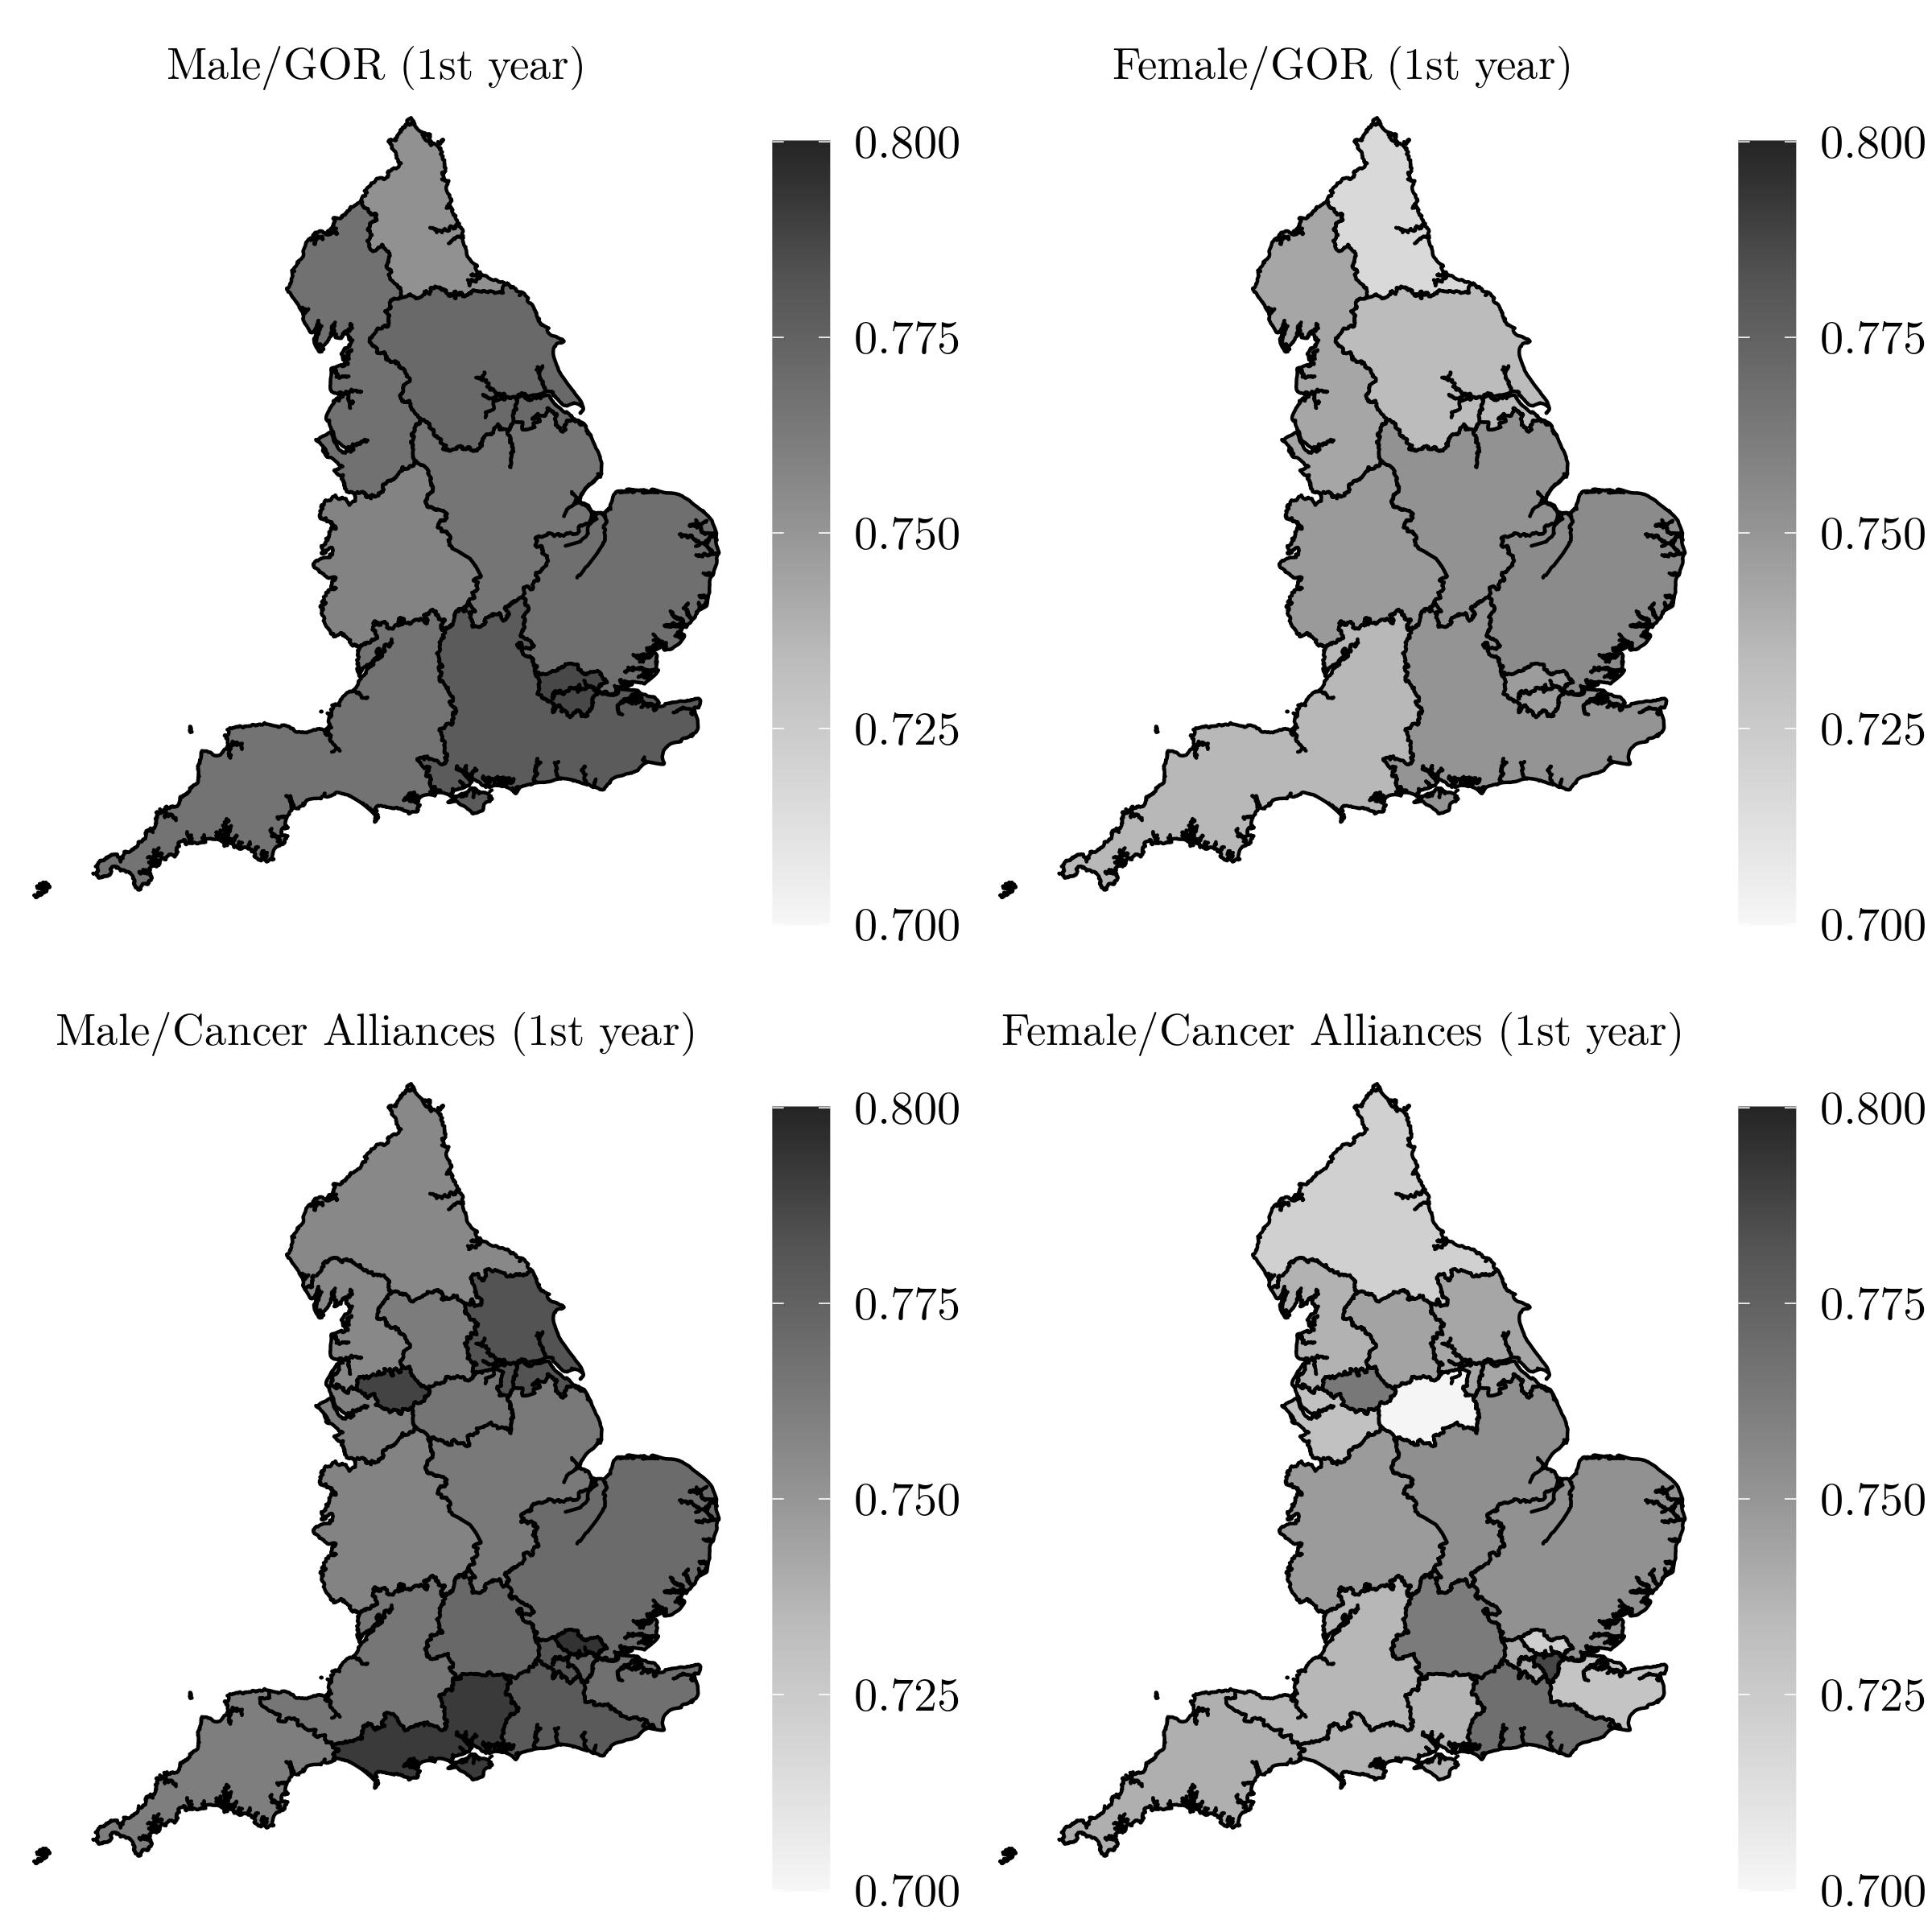
\includegraphics[width = 0.55\textwidth]{Images/cs01-t1-mean.jpg}
            \caption{Net survival point estimate for $t = 1$ with model RS-SGH LN BYM2 for all classes.}
            \label{fig:cs01-t1-mean}
        \end{figure}

    \end{frame}

    \begin{frame}[t]
		\frametitle{}
		\justifying

        \vspace{-6pt}
        \begin{figure}[!ht]
            \centering
            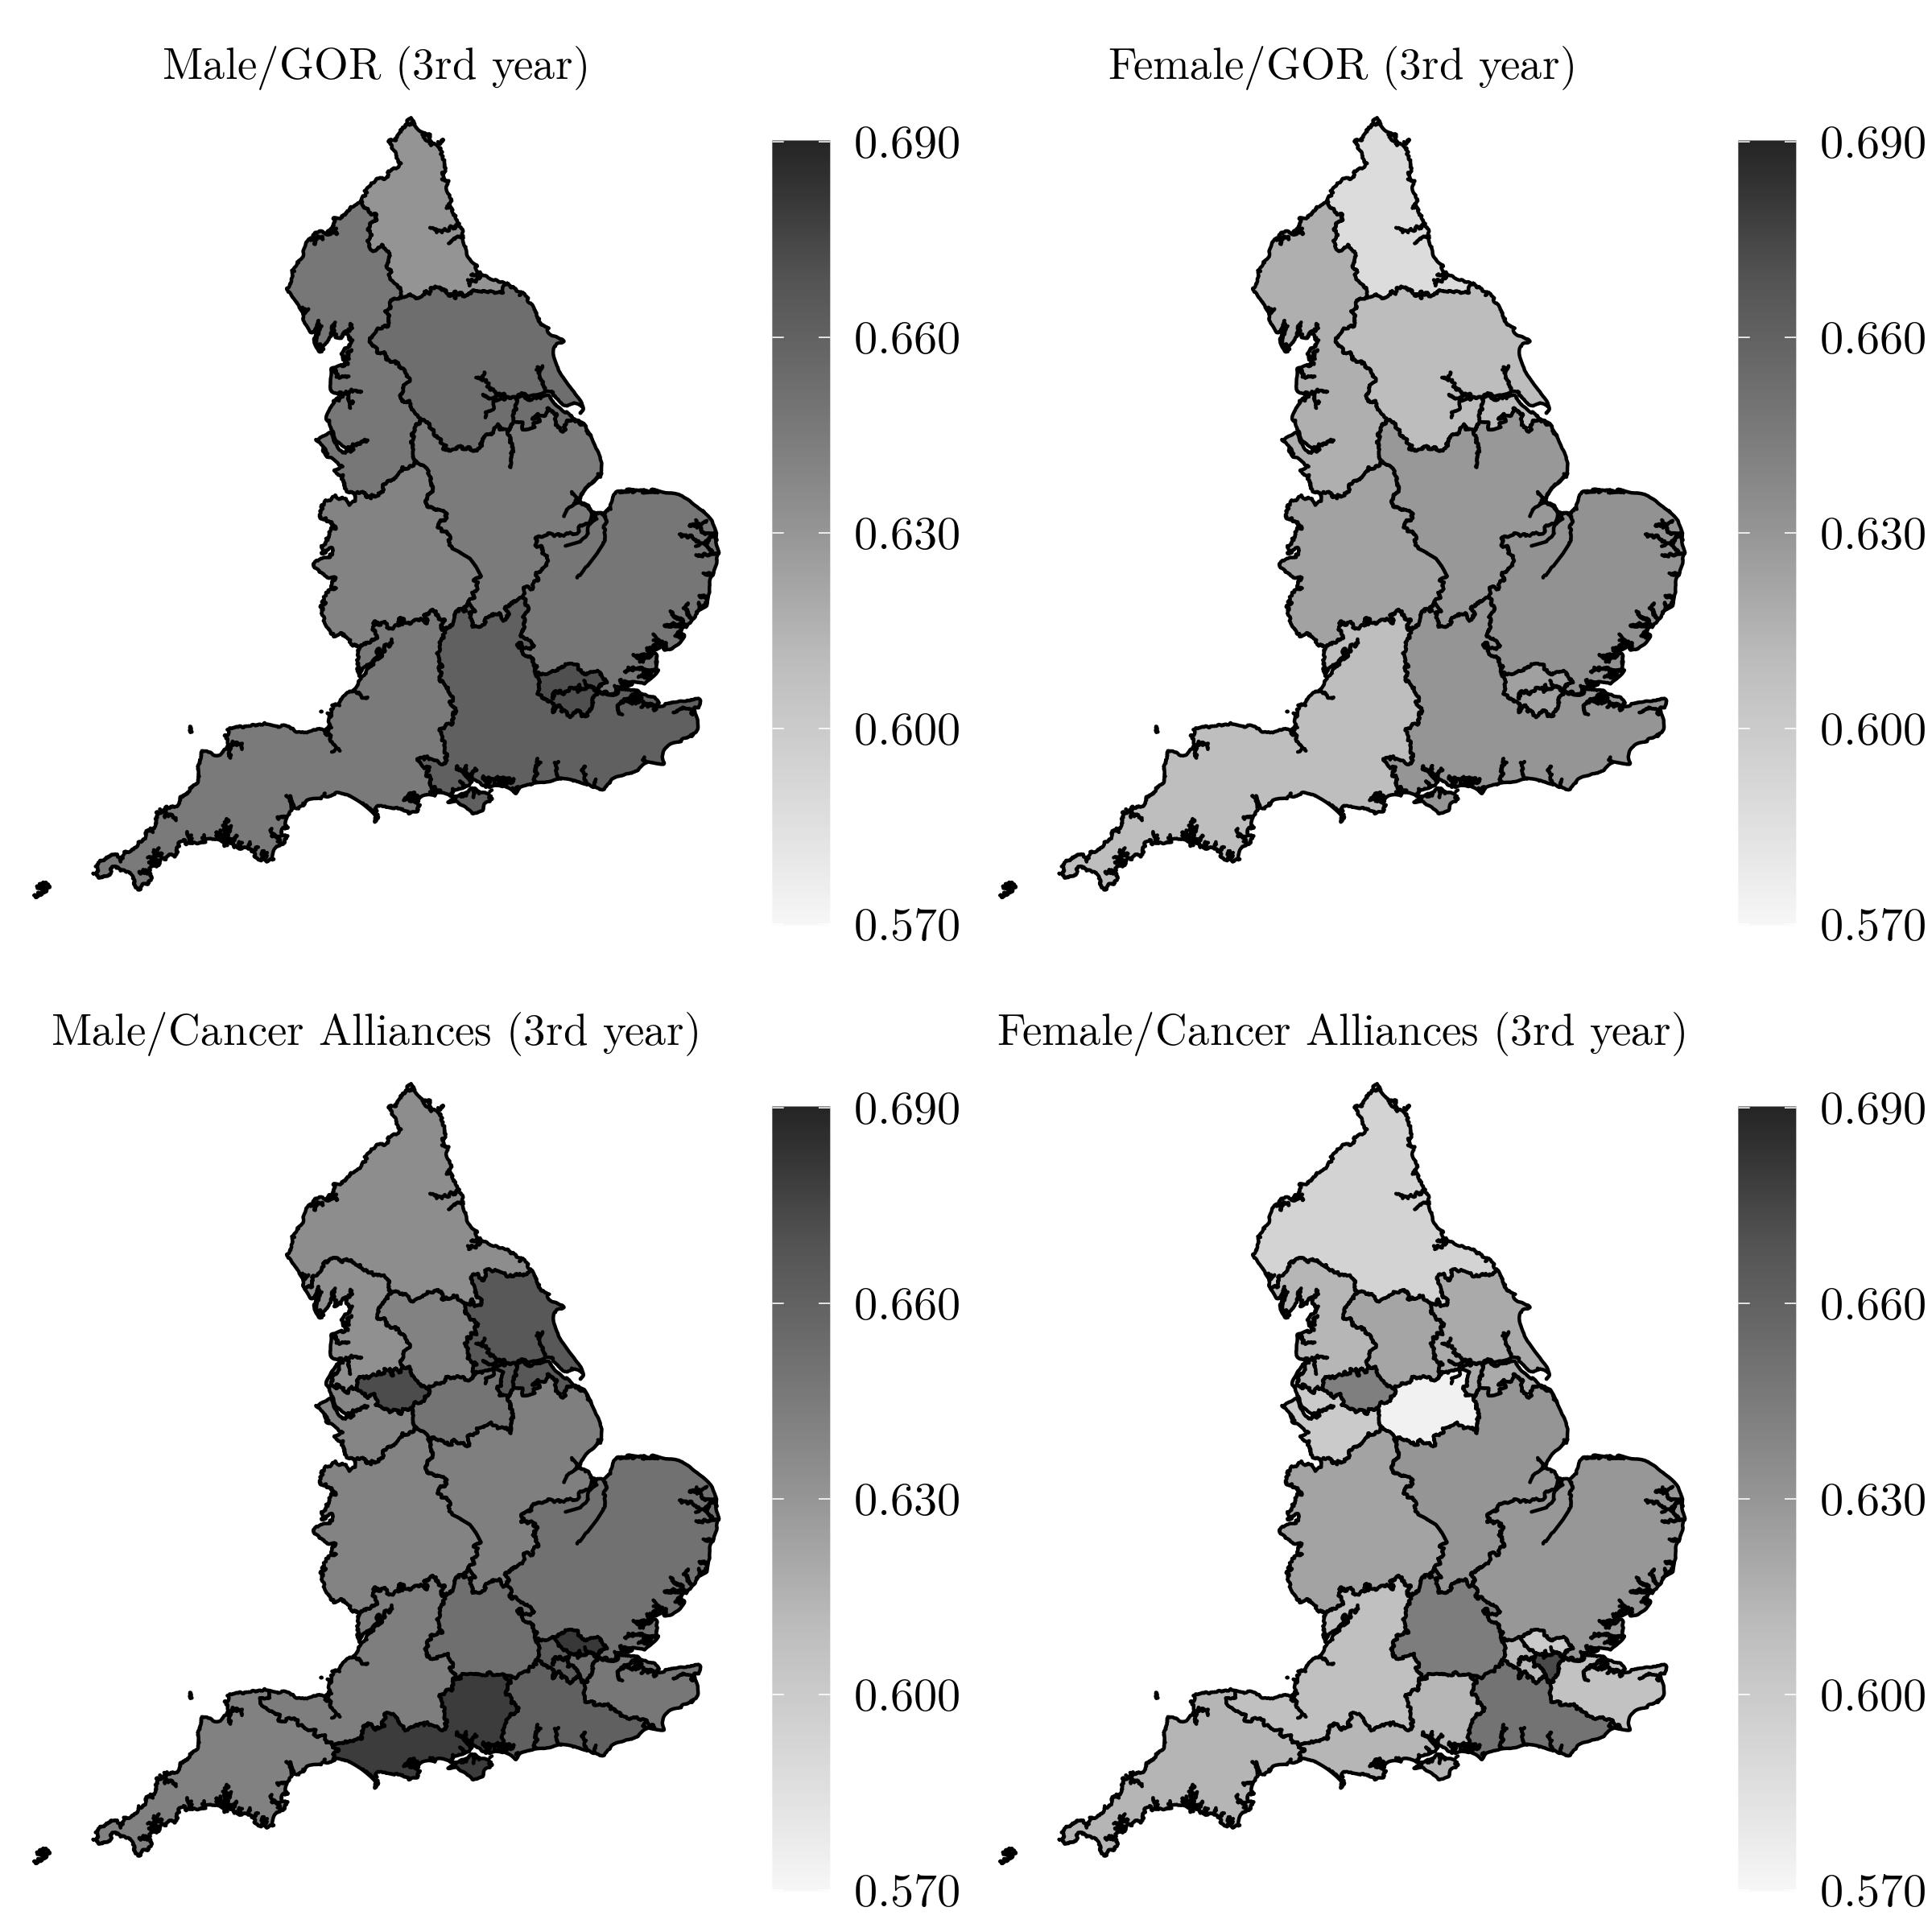
\includegraphics[width = 0.55\textwidth]{Images/cs01-t3-mean.jpg}
            \caption{Net survival point estimate for $t = 3$ with model RS-SGH LN BYM2 for all classes.}
            \label{fig:cs01-t3-mean}
        \end{figure}    

	\end{frame}

    \begin{frame}[t]
		\frametitle{}
		\justifying
        \vspace{-2pt}
        \begin{figure}[!ht]
            \centering
            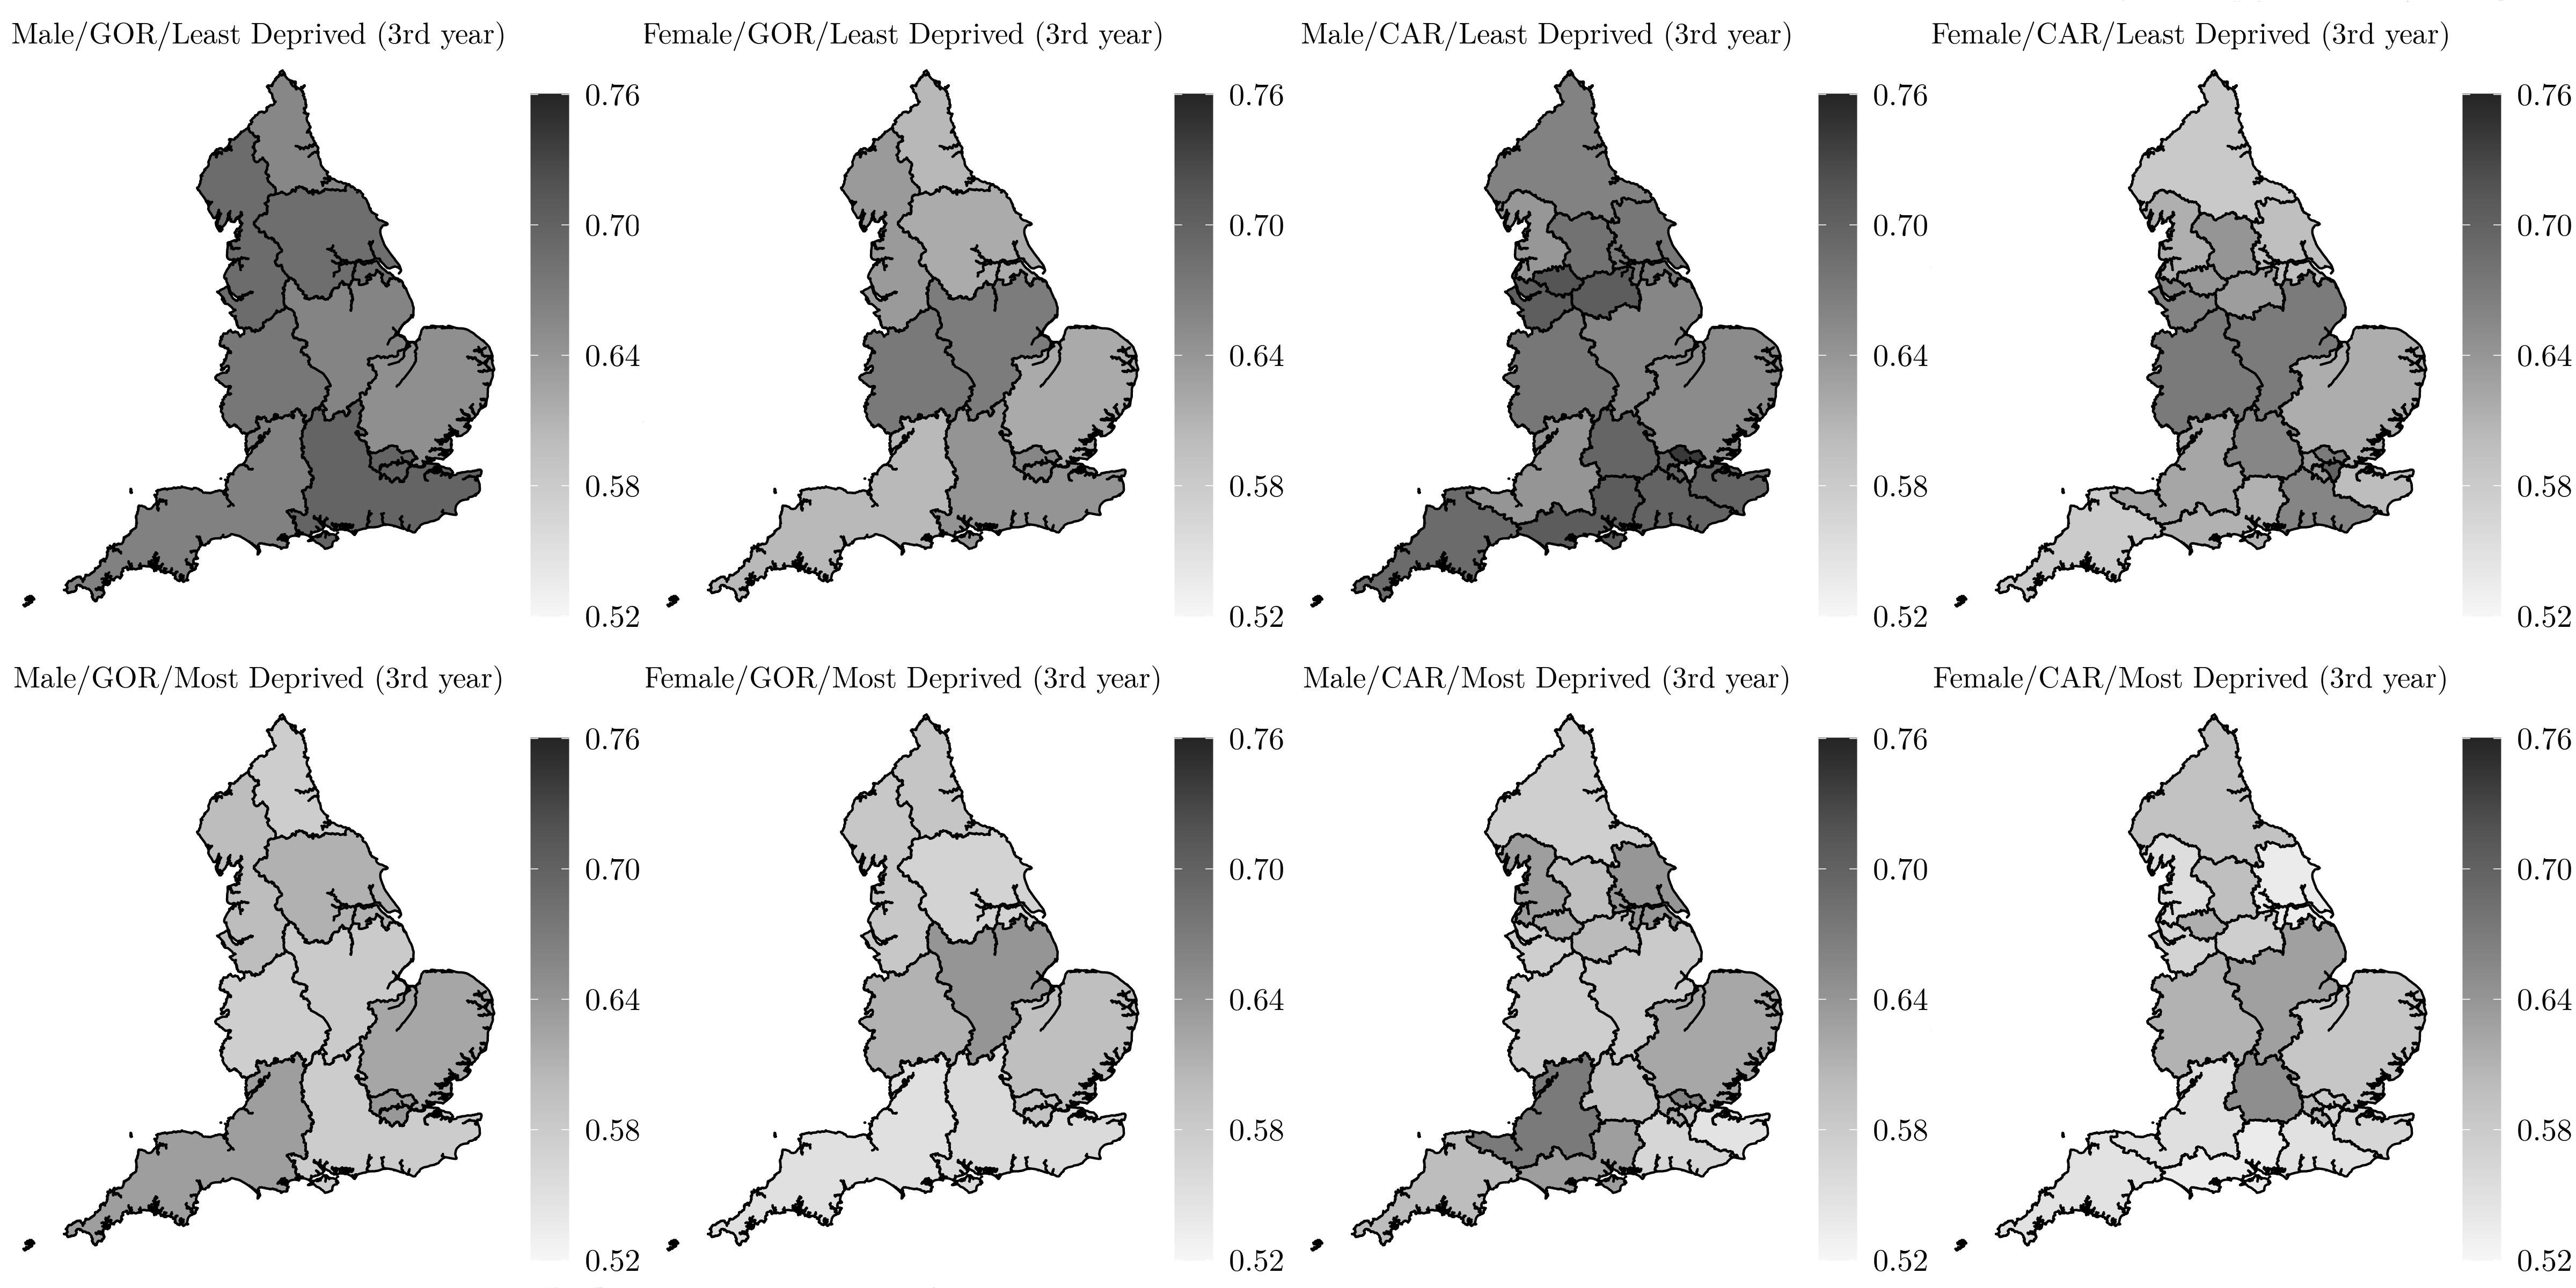
\includegraphics[width = 1\textwidth]{Images/cs01-t3-mean-dep.jpg}
            \caption{``Deprivation level'' (``1'' being \textit{least deprived} (top row) and ``5'' \textit{most deprived} (bottom row)) stratified net survival point estimate for $t = 3$ with model RS-SGH LN BYM2 for all classes.}
            \label{fig:cs01-t3-mean-dep}
        \end{figure}  
	\end{frame}

    \begin{frame}[t]
		\frametitle{}
		\justifying
        \vspace{-2pt}
        \begin{figure}[!ht]
            \centering
            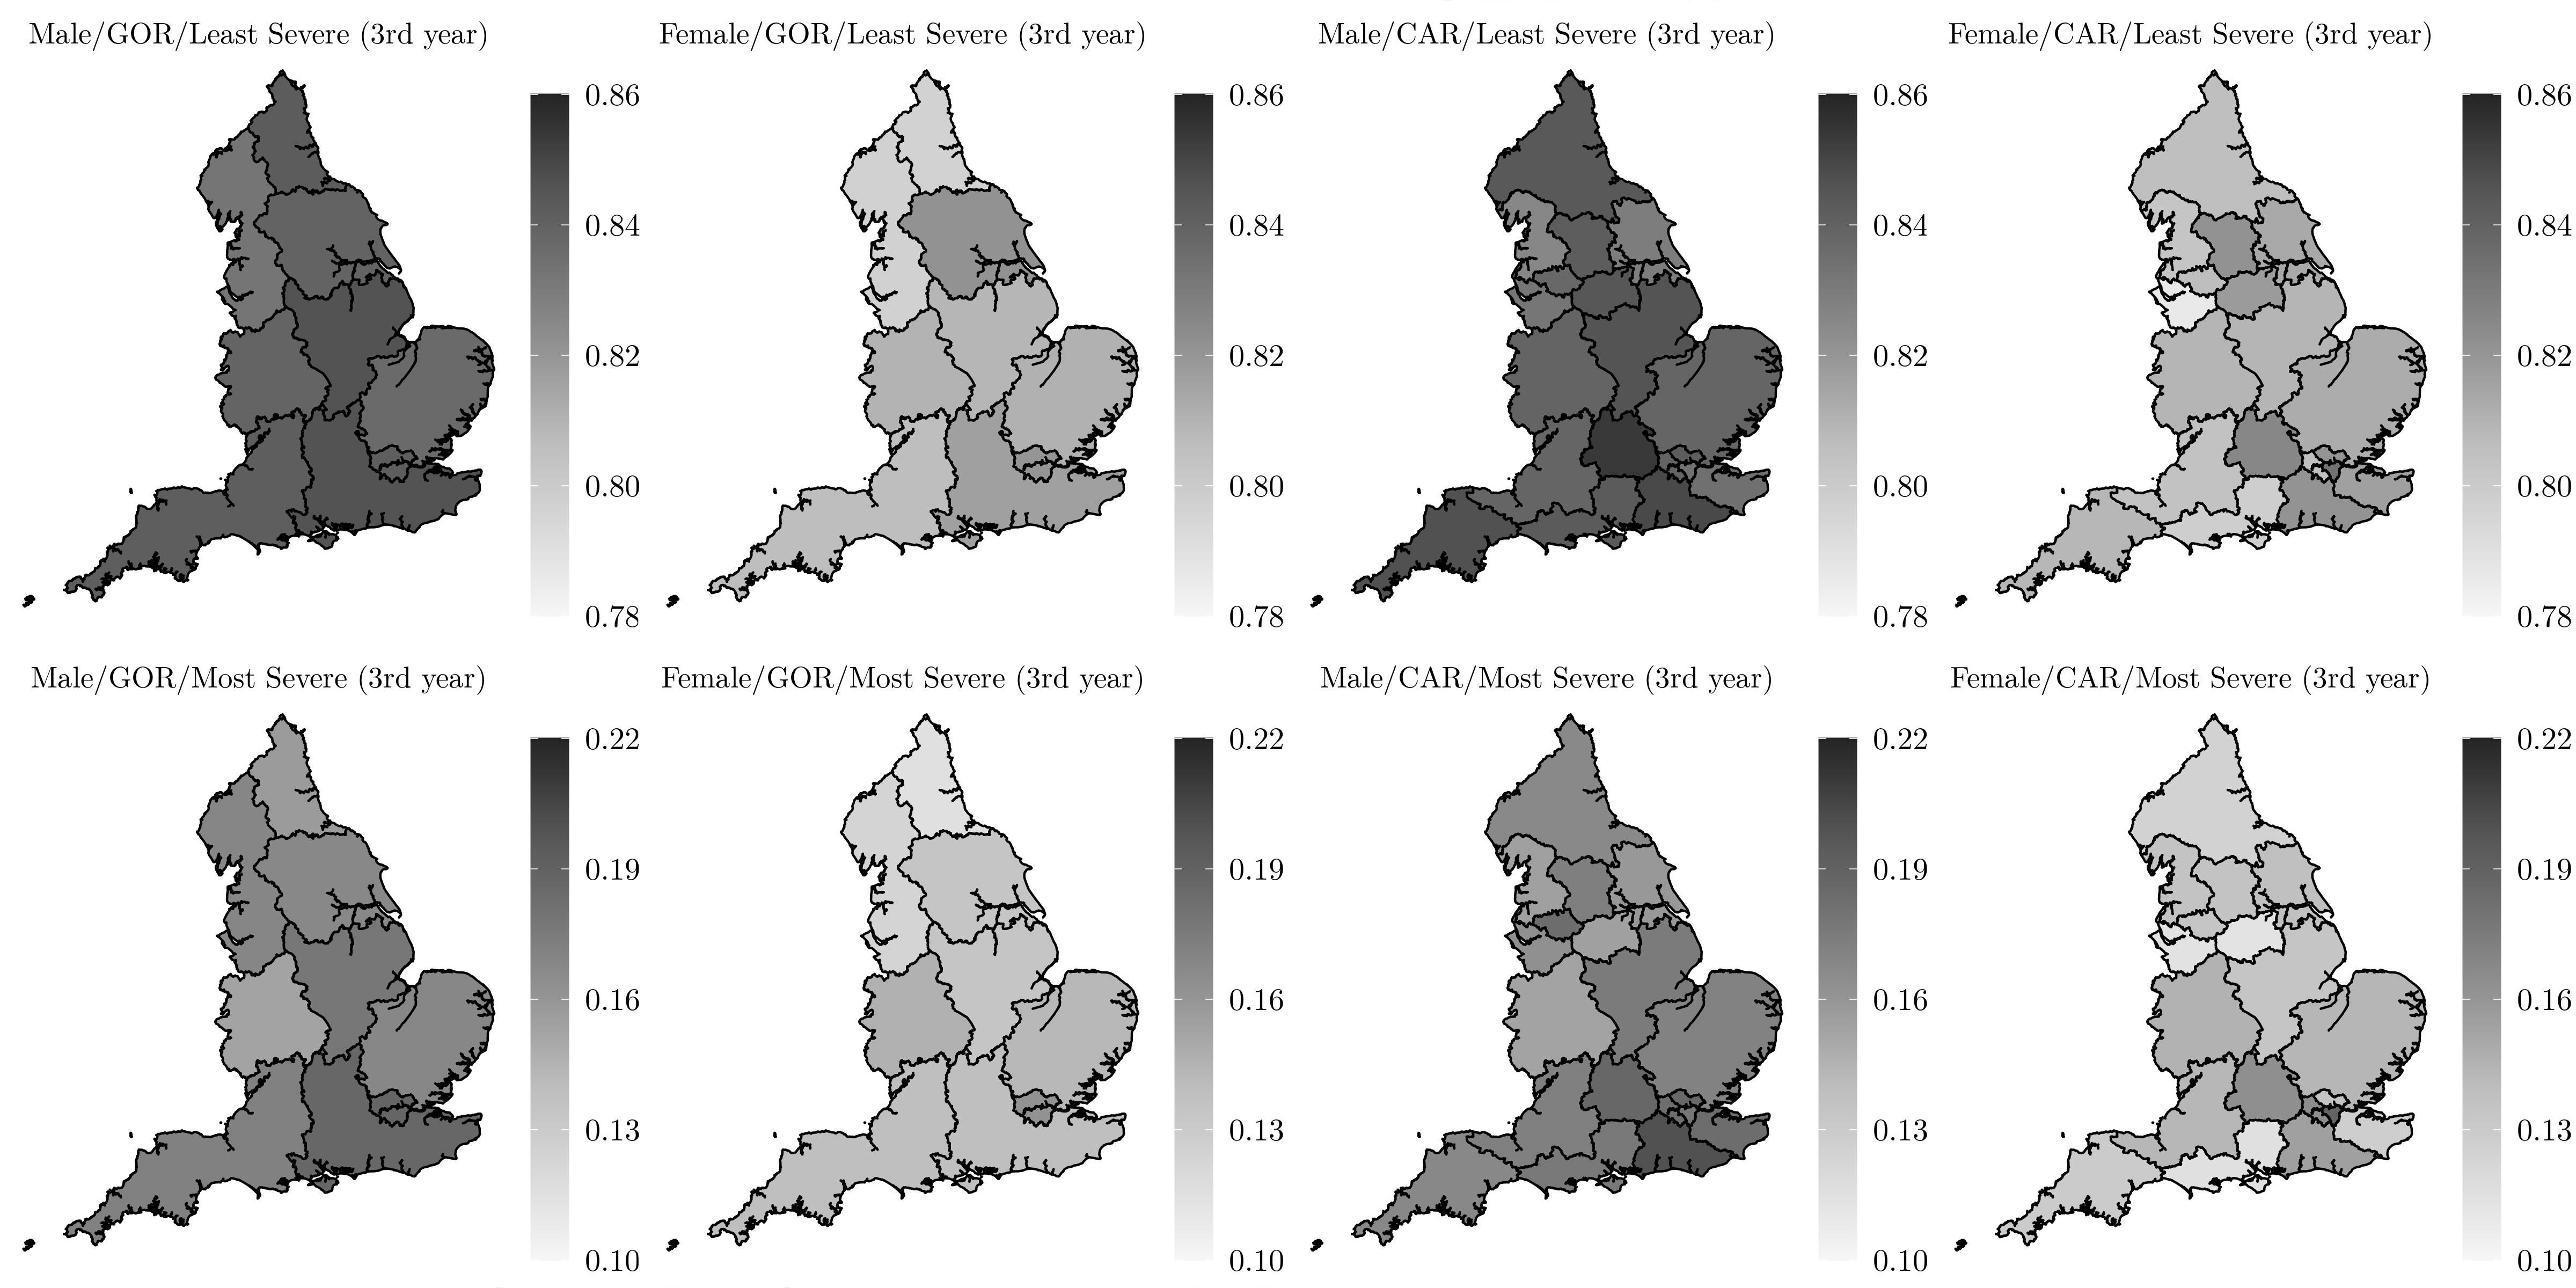
\includegraphics[width = 1\textwidth]{Images/cs01-t3-mean-cancer.jpg}
            \caption{``Cancer stage'' (``1, 2, and 3'' being \textit{least severe} (top row) and ``4'' \textit{most severe} (bottom row)) stratified net survival point estimate for $t = 3$ with model RS-SGH LN BYM2 for all classes.}
            \label{fig:cs01-t3-mean-cancer}
        \end{figure}  
	\end{frame}

    \begin{frame}[t]
		\frametitle{Case Study 02}
		\justifying

            For our second analysis, we fit \textcolor{titles}{Model \eqref{eq:exc-haz}} for $1,342$ male patients and $1,135$ female patients diagnosed in London with colon cancer in 2015 and 2016. 

            \pause
            \vspace{5pt}
            
            Our main goal is to investigate whether there seem to have differences in the net survival due to the patients' commuting habits when getting treated. 

            \pause
            \vspace{5pt}
            
            For that reason, we only account for $K = 3$ levels for cancer stage (patients with \textit{stage 4}-cancer are likely not to receive treatment for cancer removal; instead, the treatment is focused on improving their quality of life).

            \pause
            \vspace{5pt}
            
            For \textit{area of residence}, we fit models RS-SGH LL ICAR, RS-SGH LL BYM2, RS-SGH LN ICAR, RS-SGH LN BYM2, RS-SGH PGW ICAR, and RS-SGH PGW BYM2. However, for \hspace{-1pt}\textit{area of treatment}, \hspace{-1pt}we fit models \hspace{-1pt}RS-SGH LL IID,\hspace{-1pt} RS-SGH LN IID, and RS-SGH PGW IID.

            \pause
            \vspace{5pt}

            Next, as before, the best model is selected according to the $\widehat{\text{elpd}}_{\text{PSIS-LOO}}$.

	\end{frame}

    \begin{frame}[t]
		\frametitle{}
		\justifying

        \vspace{-12pt}
        \begin{figure}[!ht]
        	\centering
        	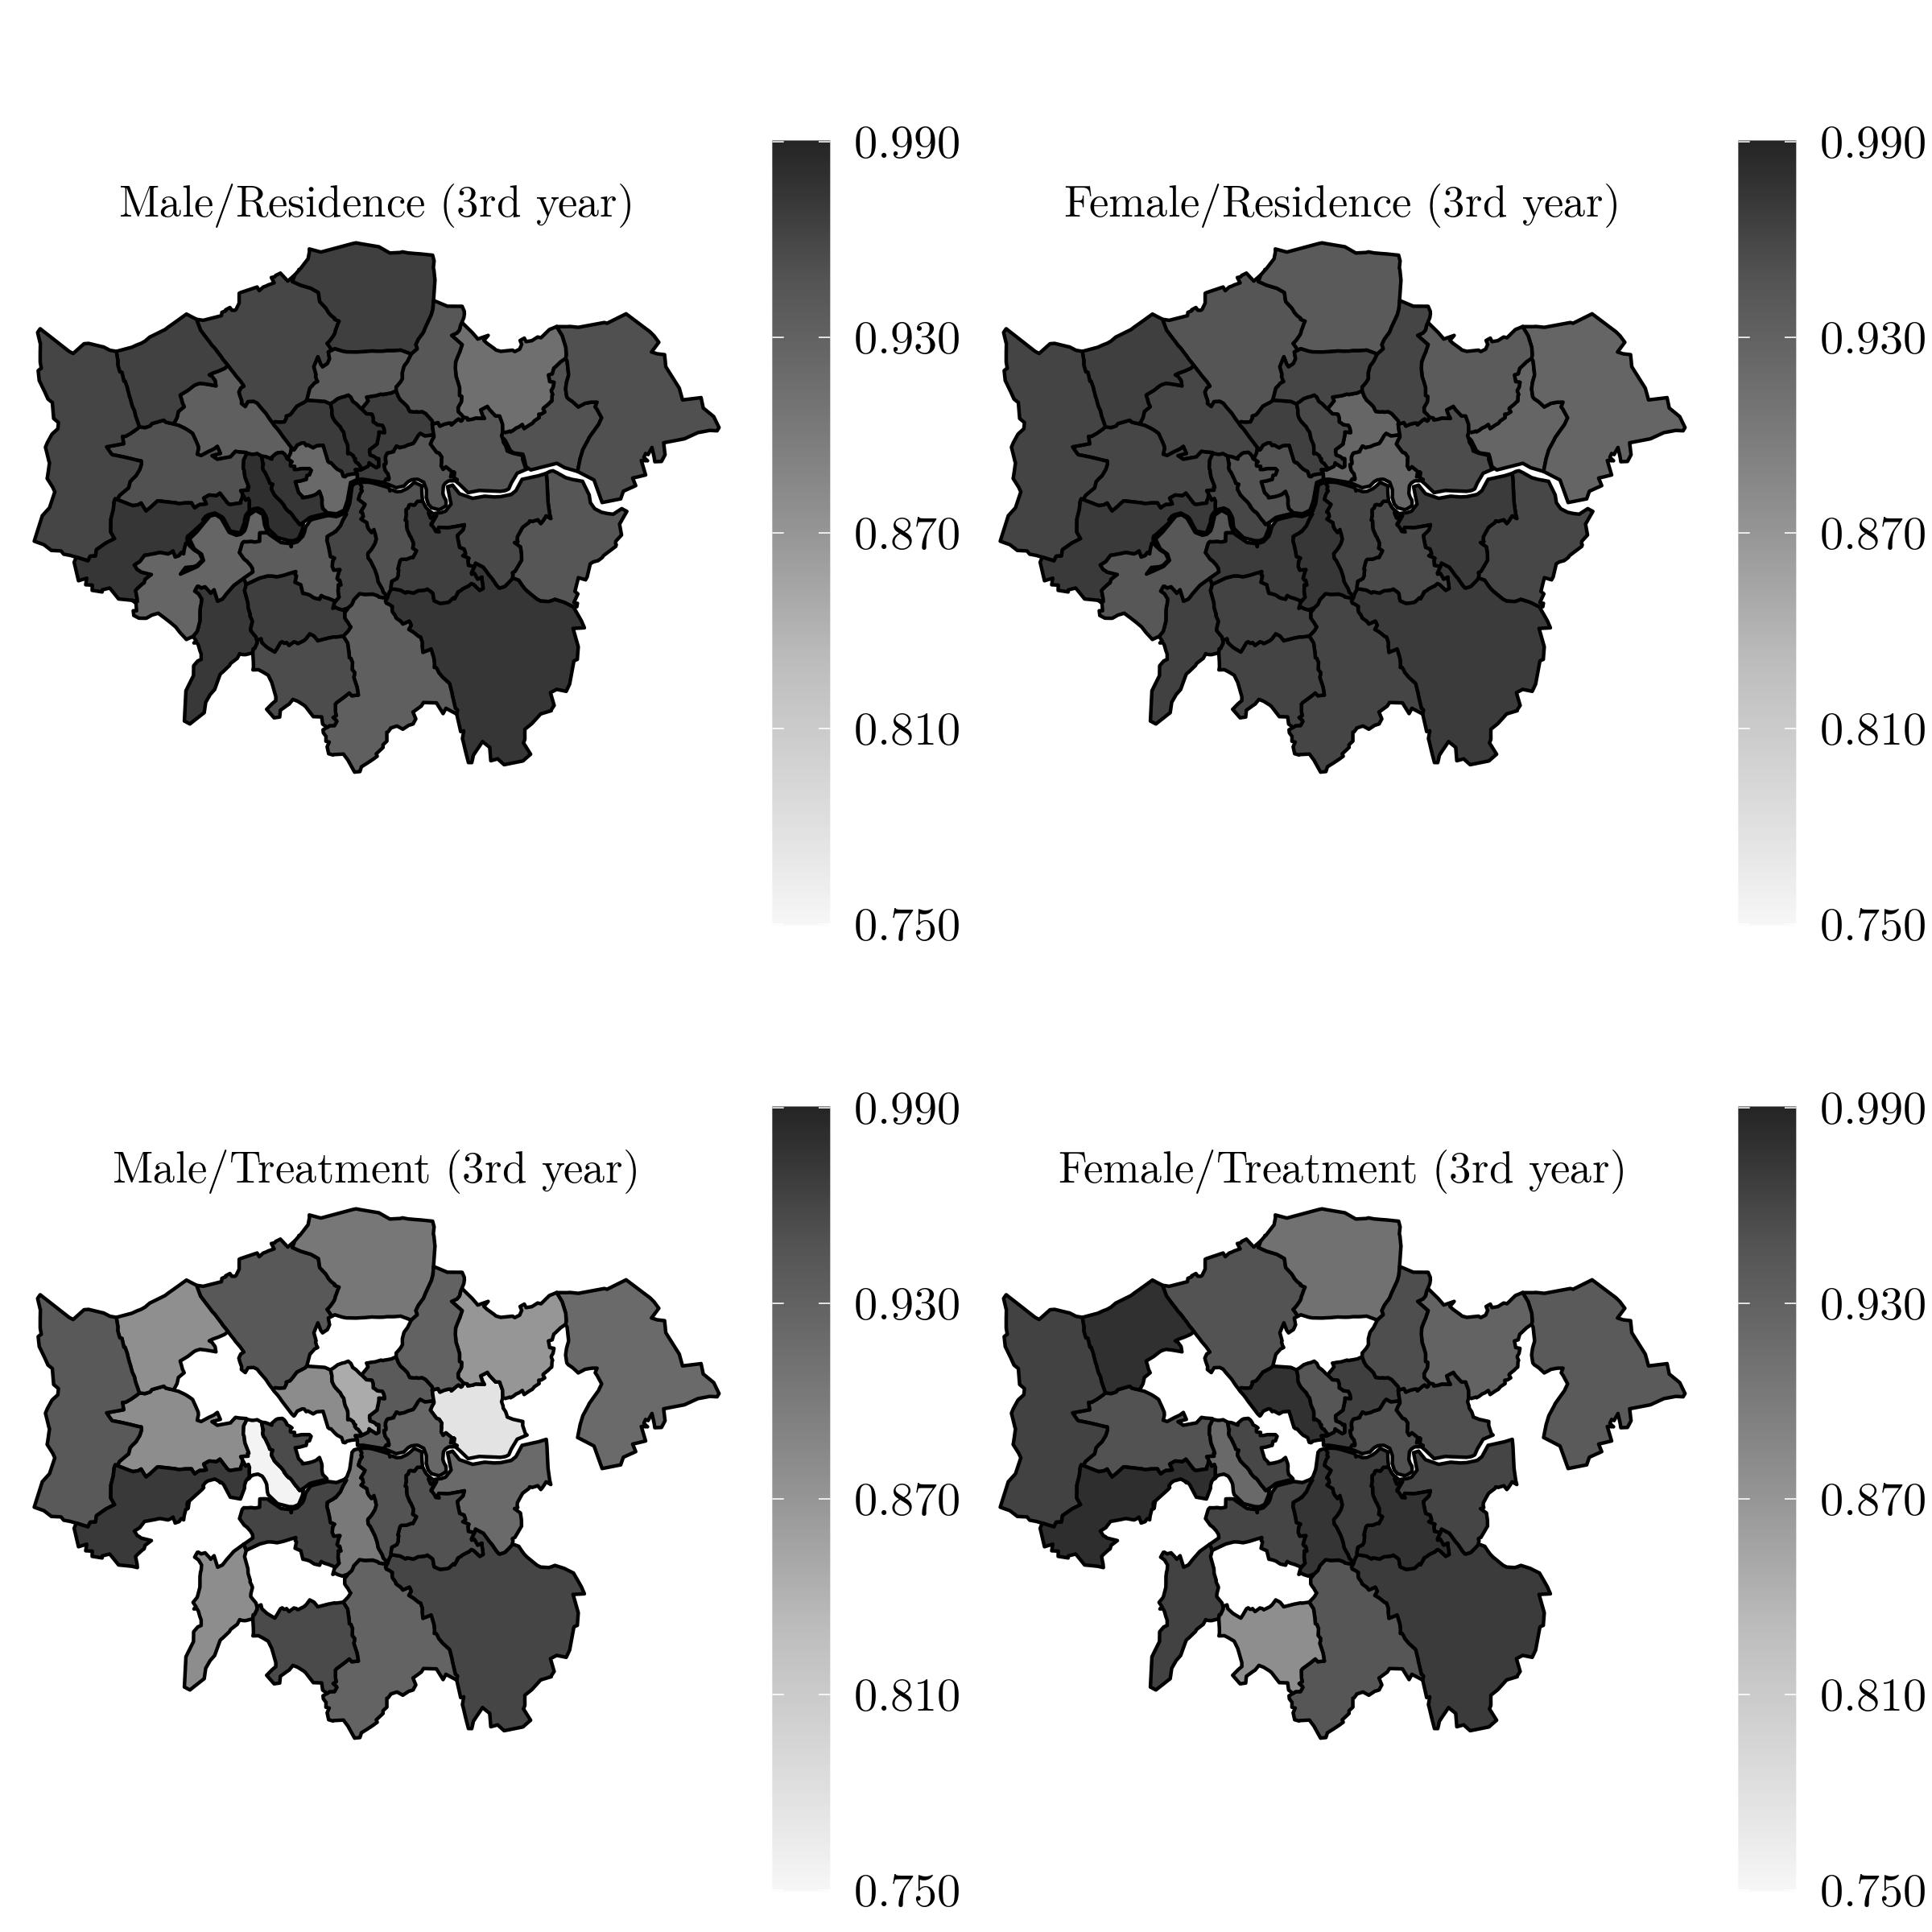
\includegraphics[width = 0.565\textwidth]{Images/cs02-t3-mean.jpg}
            \caption{Net survival point estimate for $t = 3$ with models RS-SGH PGW BYM2 and \hspace{1pt}LL IID.}
        	\label{fig:cs02-t3-mean}
        \end{figure}

	\end{frame}

    \begin{frame}[t]
		\frametitle{Discussion}
		\justifying

            We proposed the \textcolor{titles}{Relative Survival Spatial General Hazard (RS-SGH)} class of frailty models.

            \pause
            \vspace{5pt}

            This work also contains other minor contributios, such as
            \begin{enumerate} \justifying
                \item Prior distribution recommendations for the model parameters and hyperparameters.
                \item Guidelines about the sample size, baseline hazard distribution misspecification, and censoring rate when fitting models of this kind.
            \end{enumerate}

            \vspace{5pt}
            \pause
            
            In this regard, based on a  simulation study, we concluded that
            \begin{enumerate} \justifying
                \item Sample size and the censoring rate were shown to be the most important factors to control.
                \begin{enumerate} \justifying
                    \item Minimum sample size of 500--1000 patients estimate well the net survival curves.
                    \item High censoring rates (e.g., 50\%) with not large sample sizes (e.g., 200--500 patients) produced biased estimates (specially for 3-parameter distributions).
                \end{enumerate} \pause
                \item Misspecification of $h_0(\cdot)$, if we have enough non-censored data and a model that can capture the true hazard shape, had little negative impact.
            \end{enumerate}
            

            \pause
            \vspace{5pt}

            
	\end{frame}


\backupbegin
    \begin{frame}[t]
		\frametitle{}
		\justifying
  
        \vspace*{\fill} 
        \centering 
        \vspace{24pt}
        \LARGE \textcolor{titles}{Thank you!}
        \vspace*{\fill}
	\end{frame}
\backupend
 
 
\end{document}